\documentclass[../../main.tex]{subfiles}
\graphicspath{{../../image/}{../../figure/}}
\begin{document}

\section{存在性或唯一性的失效;\texorpdfstring{$\delta$}{delta} 激波与过渡波}\label{section:ch09-存在性与唯一性的失效}

\cref{theorem:ch09-严格双曲riemann解}所描绘的井然图景,一旦离开严格双曲方程组与小振幅波的领地就会崩解。

下面举例说明在构造解时可能遇到的困难。我们考虑一根无穷长多方气体柱的等熵流动,状态方程 $p=\frac{1}{\gamma}\rho^{\gamma}$, $\gamma>1$,初值如下:密度 $\bar{\rho}>0$ 沿柱长为常数;右半柱受到均匀冲量 $\bar{\rho}\bar{v}>0$,左半柱受到大小相等、方向相反的冲量 $-\bar{\rho}\bar{v}$。于是在 Lagrange 坐标下,需求解\eqref{align:ch07-p系统}的 Riemann 问题,其中 $\sigma(u)=-\frac{1}{\gamma}u^{-\gamma}$,初值为 $(u_{L},v_{L})=(\bar{u},-\bar{v})$ 与 $(u_{R},v_{R})=(\bar{u},\bar{v})$,其中 $\bar{u}=1/\bar{\rho}$。

对照\eqref{align:ch09-9-4-1}与\eqref{align:ch09-9-4-2}可知,过 $(\bar{u},-\bar{v})$ 的前向 $1$-波曲线与过 $(\bar{u},\bar{v})$ 的后向 $2$-波曲线的任一交点必在 $u_{M}>\bar{u}$ 处,因而原点处的跳跃间断被分解为两个稀疏波。在该范围内,
\begin{align}
\begin{cases}
\varphi(u;\bar{u},\bar{v})=\dfrac{2}{1-\gamma}\left(u^{\frac{1-\gamma}{2}}-w\right),&u\geqslant\bar{u},\\[2mm]
\psi(u;\bar{u},\bar{v})=-\dfrac{2}{1-\gamma}\left(u^{\frac{1-\gamma}{2}}-w\right),&u\geqslant\bar{u},
\end{cases}
\label{align:ch09-9-6-1}
\end{align}
其中已置
\begin{align}
w=\bar{u}^{\frac{1-\gamma}{2}}+\frac{1-\gamma}{2}\bar{v}.
\label{align:ch09-9-6-2}
\end{align}

解的形式取决于 $w$ 的符号。\cref{figure:ch09-气体波曲线}描绘了 $w>0$、$w=0$ 或 $w<0$ 时的波曲线。

\begin{figure}[ht]
\centering
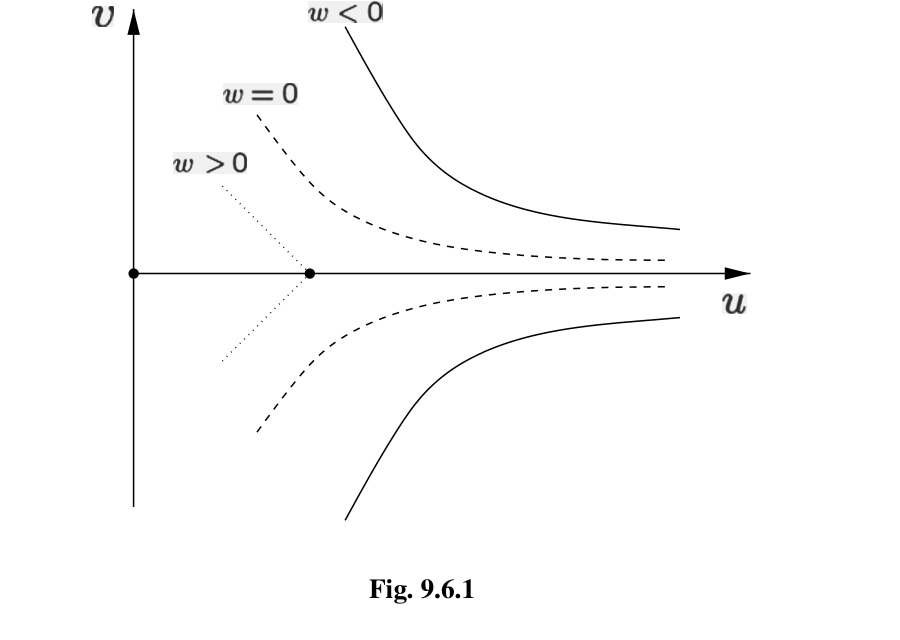
\includegraphics[width=0.7\textwidth]{ch09-fig06-01.png}
\caption{多方气体等熵流在 $u$-$v$ 平面上的波曲线: $w>0$(点线)、$w=0$(短划线)、$w<0$(实线)。}
\label{figure:ch09-气体波曲线}
\end{figure}

当 $w>0$ 时,波曲线交于 $u_{M}=w^{\frac{2}{1-\gamma}}$, $v_{M}=0$, Riemann 问题容许解
\begin{align}
(u(\xi),v(\xi))=
\begin{cases}
(\bar{u},-\bar{v}),&-\infty<\xi\leqslant-\xi_{F},\\[1mm]
\left(|\xi|^{-\frac{2}{\gamma+1}},\ -\dfrac{2}{\gamma-1}|\xi|^{\frac{\gamma-1}{\gamma+1}}+\dfrac{2}{\gamma-1}|\xi_{0}|^{\frac{\gamma-1}{\gamma+1}}\right),&-\xi_{F}<\xi\leqslant-\xi_{S},\\[2mm]
(u_{M},0),&-\xi_{S}<\xi<\xi_{S},\\[1mm]
\left(|\xi|^{-\frac{2}{\gamma+1}},\ \dfrac{2}{\gamma-1}|\xi|^{\frac{\gamma-1}{\gamma+1}}-\dfrac{2}{\gamma-1}|\xi_{0}|^{\frac{\gamma-1}{\gamma+1}}\right),&\xi_{S}\leqslant\xi<\xi_{F},\\[2mm]
(\bar{u},\bar{v}),&\xi_{F}\leqslant\xi<\infty,
\end{cases}
\label{align:ch09-9-6-3}
\end{align}
其中 $\xi_{F}=\bar{u}^{-\frac{\gamma+1}{2}}$, $\xi_{S}=w^{\frac{\gamma+1}{\gamma-1}}$。

当 $w=0$ 时,两条波曲线相交于无穷远。当 $w\downarrow0$ 时,\eqref{align:ch09-9-6-3}的 $(u(\xi),v(\xi))$ 退化为
\begin{align}
(u(\xi),v(\xi))=
\begin{cases}
(\bar{u},-\bar{v}),&-\infty<\xi\leqslant-\xi_{F},\\[1mm]
\left(|\xi|^{-\frac{2}{\gamma+1}},\ \dfrac{2}{\gamma-1}\operatorname{sgn}\xi\,|\xi|^{\frac{\gamma-1}{\gamma+1}}\right),&-\xi_{F}<\xi<\xi_{F},\\[2mm]
(\bar{u},\bar{v}),&\xi_{F}\leqslant\xi<\infty.
\end{cases}
\label{align:ch09-9-6-4}
\end{align}
注意 $u$ 在 $\xi=0$ 处的奇性可积,而 $v$ 连续。容易验证:由\eqref{align:ch09-9-6-4}定义的 $(u(\xi),v(\xi))$ 在分布意义下满足\eqref{align:ch09-9-1-3},对\eqref{align:ch07-p系统}即
\begin{align}
\begin{cases}
(-v-\xi u)^{\cdot}+u=0,\\[1mm]
\left(\dfrac{1}{\gamma}u^{-\gamma}-\xi v\right)^{\cdot}+v=0,
\end{cases}
\label{align:ch09-9-6-5}
\end{align}
从而求解了 $w=0$ 的 Riemann 问题。$u(0)=\infty$ 仅意味着密度 $\rho$ 沿直线 $x=0$ 为零。

当 $w<0$ 时,两条波曲线甚至在无穷远处也不相交,因而构造不出 Riemann 问题的标准解。当然物理问题仍可解。事实上,可在 Euler 坐标下把它重新表述为\eqref{align:ch07-理想气体}(其中 $\kappa=1/\gamma$)的 Riemann 问题,初值为: $\rho(x,0)=\bar{\rho}$, $x\in(-\infty,\infty)$; $v(x,0)=-\bar{v}$, $x\in(-\infty,0)$; $v(x,0)=\bar{v}$, $x\in(0,\infty)$。该解由两个稀疏波组成,其尾端彼此后退,速度分别为 $\pm\frac{2}{\gamma-1}w$,在二者之间留下一个 $\rho$ 为零的真空区。\cref{section:ch02-平衡律}的讨论不覆盖此流动到 Lagrange 坐标的映射,因为形变梯度的行列式 $\rho^{-1}$ 在真空态上无界。事实上,在该坐标变换下,物理时空中真空态所占的整个扇形区域被映射到参考时空中的单一直线 $x=0$。因而 $u=\rho^{-1}$ 在 $\xi=0$ 处变得非常奇异:
\begin{align}
(u(\xi),v(\xi))=
\begin{cases}
(\bar{u},-\bar{v}),&-\infty<\xi\leqslant-\xi_{F},\\[1mm]
\left(|\xi|^{-\frac{2}{\gamma+1}}-\dfrac{4}{\gamma-1}w\delta_{0},\ \dfrac{2}{\gamma-1}\operatorname{sgn}\xi\left[|\xi|^{\frac{\gamma-1}{\gamma+1}}-w\right]\right),&-\xi_{F}<\xi<\xi_{F},\\[3mm]
(\bar{u},\bar{v}),&\xi_{F}\leqslant\xi<\infty,
\end{cases}
\label{align:ch09-9-6-6}
\end{align}
其中 $\delta_{0}$ 表示原点处的 Dirac $\delta$ 函数。事实上,若把 $u^{-\gamma}(\xi)$ 视为在原点 $\xi=0$ 处为零的连续函数,则\eqref{align:ch09-9-6-6}的 $(u(\xi),v(\xi))$ 是\eqref{align:ch09-9-6-5}的分布解。在 $(x,t)$ 坐标下,\eqref{align:ch09-9-6-6}在 $u$ 上诱导出沿 $t$ 轴的静止奇性 $-\frac{4}{\gamma-1}wt\delta_{0}$。这种承载点质量的新型奇性称为\emph{$\delta$ 激波}。

有人会争辩: $\delta$ 激波的出现是因为我们采用了 Lagrange 坐标,而它并不适合此问题。然而事实证明, $\delta$ 激波经常出现在 Riemann 问题的解中,尤其是对非严格双曲方程组。相关文献见\cref{section:ch09-注记}。正如我们在\cref{section:ch09-粘性波扇}中将看到的,消失粘性方法有助于洞察 $\delta$ 激波的形成。

严格双曲性的失效也是 Riemann 问题解不唯一的一个根源。Liu $E$ 条件不再充分筛选出唯一解。为说明这一点,考虑模型方程组\eqref{align:ch07-脐点模型}的 Riemann 问题,初值 $(u_{L},v_{L})=(1,0)$、$(u_{R},v_{R})=(a,0)$,其中 $a\in(-\frac{1}{2},0)$。一个解由两个常值状态 $(1,0)$ 与 $(a,0)$ 组成,二者由一个过压缩激波连接,速度 $s=1+a+a^{2}$,满足 Liu $E$ 条件。然而还有另一个解,由三个常值状态 $(1,0)$、$(-1,0)$、$(a,0)$ 组成,其中 $(-1,0)$ 与 $(1,0)$ 由一个速度为 $1$ 的 $1$-接触间断连接,而 $(a,0)$ 与 $(-1,0)$ 由一个速度 $s=1-a+a^{2}$ 的 $2$-激波连接。两个激波都满足 Liu $E$ 条件。按\cref{section:ch08-黏性激波剖面}对此方程组的讨论,人们可能倾向于取消过压缩激波的资格,此时 Riemann 问题的第二个解就成为容许解。这当然取决于\eqref{align:ch08-模型黏性}是否为\eqref{align:ch07-脐点模型}的适当耗散形式这一前提。

非唯一性问题也出现在容许欠压缩激波的(通常非严格双曲)方程组中。为确定起见,考虑这样一个两个守恒律的方程组。任一欠压缩激波被来自右方的 $1$-特征与来自左方的 $2$-特征同时穿过。因而,这类激波可被并入一个波扇,其左侧含一个压缩 $1$-激波或 $1$-稀疏波,右侧含一个压缩 $2$-激波或 $2$-稀疏波。在这种作用下,欠压缩激波充当连接两个特征族的"桥",故称为\emph{过渡波}。也可能有过渡稀疏波,它们是 $1$-稀疏波与 $2$-稀疏波的复合。当 $1$-稀疏波曲线与 $2$-稀疏波曲线在严格双曲性失效的线 $\lambda_{1}(U)=\lambda_{2}(U)$ 上相切相遇时,就可能出现这种波。纳入过渡波的可能使 Riemann 问题解族更丰富,从而使唯一性问题更棘手。正如\cref{chapter:ch08-容许激波}所指出,粘性或粘性-毛细条件以及动力学关系正被用作这些欠压缩激波的容许准则。此时再怎么强调处理真实物理方程组的重要性也不为过。

\end{document}
